\documentclass[t,aspectratio=169]{beamer}
%\usetheme{Berkeley}
\usepackage{graphicx}
\usepackage{amsmath}
\usepackage[american]{circuitikz}

\title{Clase 28}
\subtitle{Modelo digital del MOSFET}
\author{Dr.-Ing. Juan José Montero Rodríguez}
\subject{Elementos Activos}
\institute{Escuela de Ingeniería Electrónica}
\date{Semestre II-2023}

\begin{document}

\begin{frame}{}
\maketitle
\end{frame}


\section{Modelo ideal}
\begin{frame}{Niveles lógicos en transistores MOSFET}

En circuitos digitales, la entrada puede ser un $0$ lógico o un $1$ lógico.

\begin{figure}[H]
    \centering
    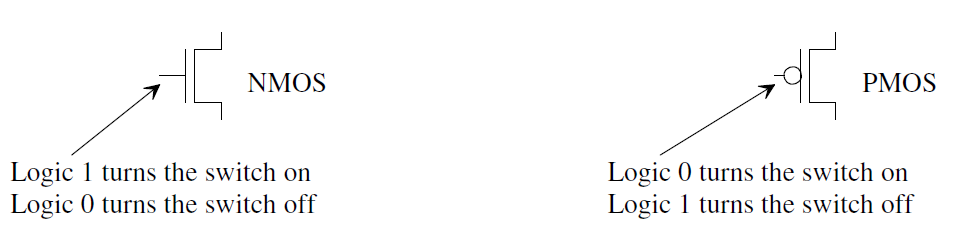
\includegraphics[width=0.8\textwidth]{figuras/mosfet_as_a_switch.png}
\end{figure}

Los niveles lógicos dependen de la tensión de alimentación.

\begin{itemize}
    \item $1 = V_{DD}$
    \item $0 = GND$
\end{itemize}

Se considera un $1$ lógico si $V_{GS} > V_{DD}/2$.

Se considera un $0$ lógico si $V_{GS} < V_{DD}/2$.

\end{frame}

\begin{frame}{El transistor MOSFET como interruptor}

Considere el circuito digital que se muestra en la figura.

\begin{itemize}
    \item En el instante $t=0$ la tensión de entrada pasa de $0$ a $V_{DD}$.
    \item El condensador se empieza a descargar a través del MOSFET.
\end{itemize}

\begin{figure}
    \centering
    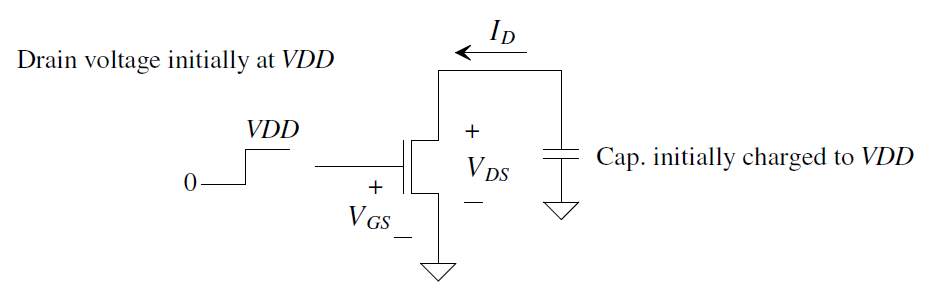
\includegraphics[width=0.8\textwidth]{figuras/mosfet_circuito_digital.png}
\end{figure}

La descarga no es instantánea, el transistor tarda cierto tiempo en pasar la salida de un $1$ lógico a un $0$ lógico.

\end{frame}


\begin{frame}{Modelo digital del MOSFET (ideal)}

El transistor se puede describir como un interruptor en serie con una resistencia.

\begin{itemize}
	\item El interruptor es ideal y conmuta en $V_{DD}/2$.
	\item La resistencia de conmutación es la que limita la velocidad de carga/descarga.
\end{itemize}

\begin{figure}
    \centering
    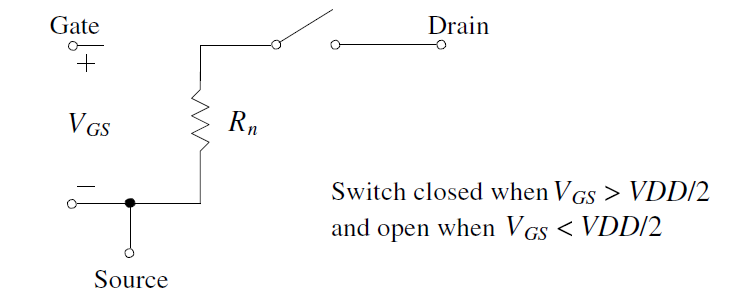
\includegraphics[width=0.7\textwidth]{figuras/mosfet_modelo_digital.png}
\end{figure}

La constante de tiempo $\tau = RC$ limita la velocidad de operación de los circuitos digitales.

\end{frame}


\begin{frame}{Resistencia de conmutación}

Para calcular la resistencia de conmutación se toman los valores finales e iniciales de tensión y corriente, como se muestra en el gráfico:
%
\begin{figure}
    \centering
    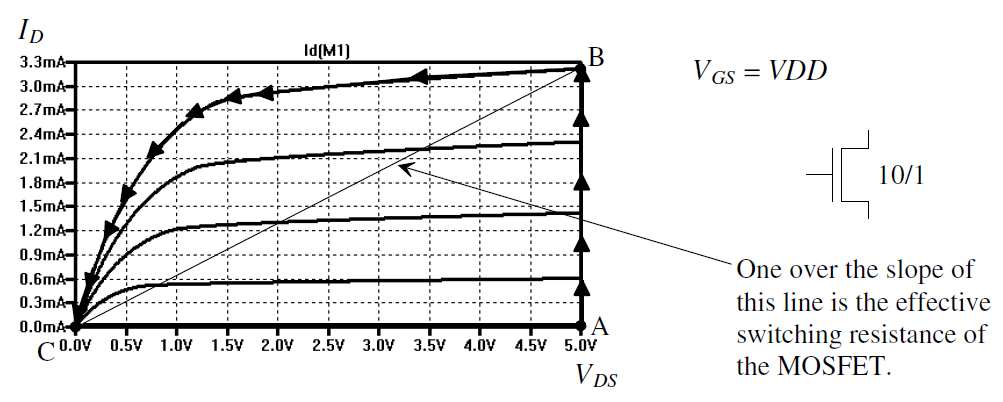
\includegraphics[width=0.8\textwidth]{figuras/mosfet_curva_salida_digital.png}
\end{figure}
%
\[ R_n = \left( \dfrac{\Delta I_D}{\Delta V_{DS}} \right)^{-1} = \dfrac{V_{DD}}{\dfrac{1}{2} K' \dfrac{W}{L} (V_{DD}-V_{TH})^2} = \dfrac{V_{DD}}{I_{D,sat}} =  R_n' \cdot \dfrac{L}{W} \]

\end{frame}


\section{Capacitancias}
\begin{frame}{Capacitancias parásitas del MOSFET}
\centering
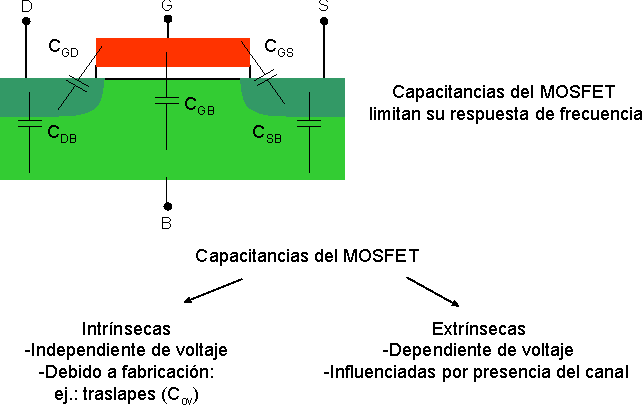
\includegraphics[width=11cm]{./figuras/MOScap.pdf}
\end{frame}


\begin{frame}{Capacitancias del MOSFET en lineal y en saturación}
\centering
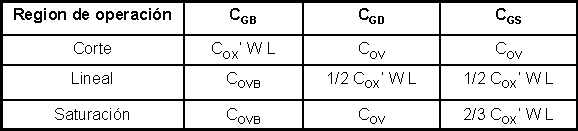
\includegraphics[width=10cm]{./figuras/captable.pdf}

\vspace{3mm}
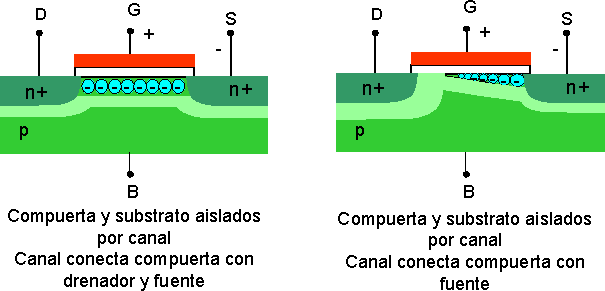
\includegraphics[width=10cm]{./figuras/MOScap2.pdf}
\end{frame}


\begin{frame}{Capacitancia de Miller}

Para comprender los efectos capacitivos, considere primero lo siguiente:

\vspace{-3mm}
\begin{columns}

\begin{column}{0.5\textwidth}

\centering
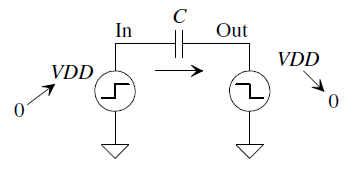
\includegraphics[width=0.8\textwidth]{figuras/miller1.png}

\end{column}

\begin{column}{0.5\textwidth}

\[ Q_{init} = C \cdot (0 - V_{DD}) = -C \cdot V_{DD} \]
\[ Q_{final} = C \cdot (V_{DD} - 0) = +C \cdot V_{DD} \]

\end{column}

\end{columns}

\vspace{3mm}
El circuito puede dividirse en un circuito de entrada y un circuito de salida con el doble de la capacitancia:

\begin{columns}

\begin{column}{0.6\textwidth}

\centering
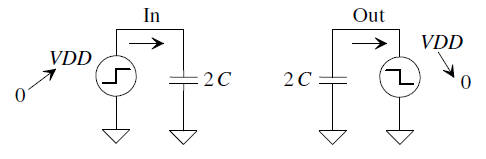
\includegraphics[width=\textwidth]{figuras/miller2.png}

\end{column}

\begin{column}{0.4\textwidth}

\[ Q_{total} = Q_{final} - Q_{inicial} \]
\[ Q_{total} = 2C \cdot V_{DD} \]

\end{column}

\end{columns}

\end{frame}


\section{Modelo capacitivo}
\begin{frame}{Modelo del MOSFET con condensadores parásitos}

\vspace{-5mm}
\begin{columns}

\begin{column}{0.5\textwidth}

Asuma que la capacitancia entre compuerta y drenador, así como la capacitancia entre compuerta y surtidor es 0.5C\textsubscript{OX} (operación en la zona lineal).

\vspace{3mm}
Esta es una sobreestimación del valor de la capacitancia, para calcular el peor de los casos.

\vspace{3mm}
La capacitancia entre compuerta y drenador conecta la entrada con la salida.

\vspace{3mm}
Separando la capacitancia entre compuerta y drenador en una capacitancia equivalente entre la entrada y tierra, y la salida y tierra se tiene el circuito de la derecha.

\end{column}

\begin{column}{0.5\textwidth}

\centering
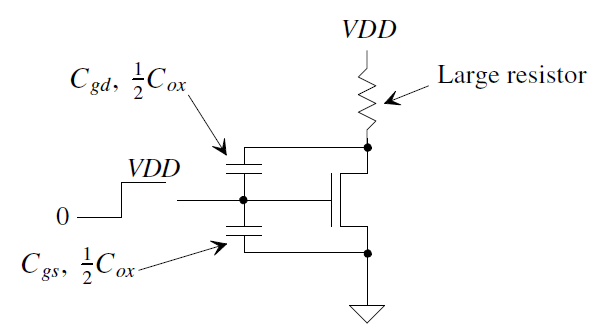
\includegraphics[width=0.8\textwidth]{figuras/mosfet_capacitancias_cgs_cgd.png}

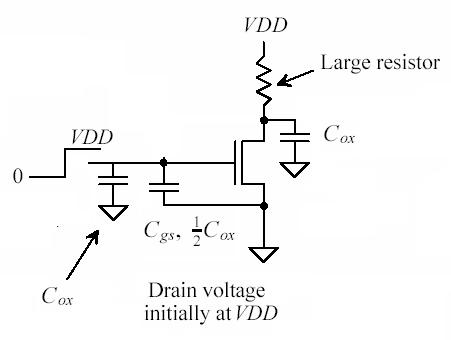
\includegraphics[width=0.8\textwidth]{figuras/digital5.png}

\end{column}

\end{columns}

\end{frame}


\begin{frame}{Modelo digital del MOSFET (con condensadores parásitos)}

El modelo equivalente incluyendo efectos capacitivos:

\centering
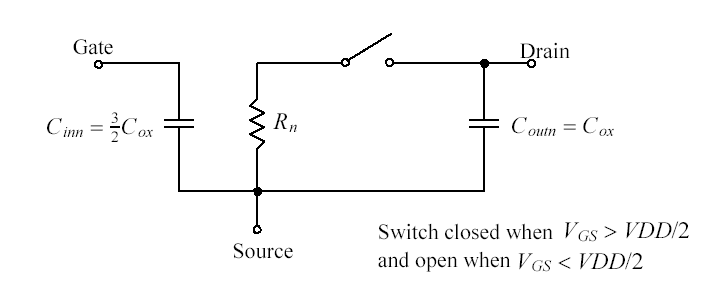
\includegraphics[width=10cm]{./figuras/digital6.png}

\begin{columns}

\begin{column}{0.5\textwidth}

\[ C_{inn} = C_{gs} + 2C_{gd} = \dfrac{3}{2} C_{OX} \]
%
\[ C_{outn} = 2C_{gd} = C_{OX} \]

\end{column}

\begin{column}{0.5\textwidth}

\[ R_{n} \approx 15\ k\Omega \cdot L/W \]
\[ R_{p} \approx 45\ k\Omega \cdot L/W \]

\end{column}

\end{columns}

\end{frame}


\begin{frame}{Retardo y tiempo de transición}

\begin{figure}[H]
    \centering
    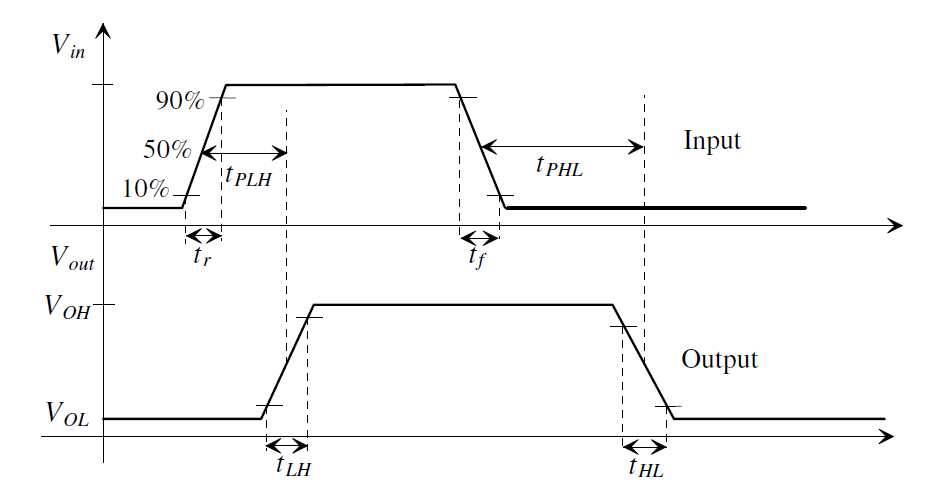
\includegraphics[width=0.7\textwidth]{figuras/mos_pass_gate_delay_and_transition.png}
\end{figure}

\vspace{-5mm}
\[ t_{delay} = t_{PLH} = t_{PHL} = 0.7 RC \]
\[ t_{r} = t_{f} = 2.2 RC \]

\end{frame}


\begin{frame}{Retardo y tiempo de transición: definiciones}

En el diagrama de la diapositiva anterior se definen los siguientes parámetros:

\begin{itemize}
    \item $t_{HL}$: tiempo que tarda la salida en pasar de $V_{OH}$ a $V_{OL}$.
    \item $t_{LH}$: tiempo que tarda la salida en pasar de $V_{OL}$ a $V_{OH}$.
    \item $t_{PLH}$: retardo (delay) de entrada a salida, cuando la entrada pasa de bajo a alto (medido en 50\%).
    \item $t_{PHL}$: retardo (delay) de entrada a salida, cuando la entrada pasa de alto a bajo (medido en 50\%).
\end{itemize}

\end{frame}


\section{Inversores}
\begin{frame}{El inversor NMOS}

\vspace{-5mm}
\begin{figure}
    \centering
    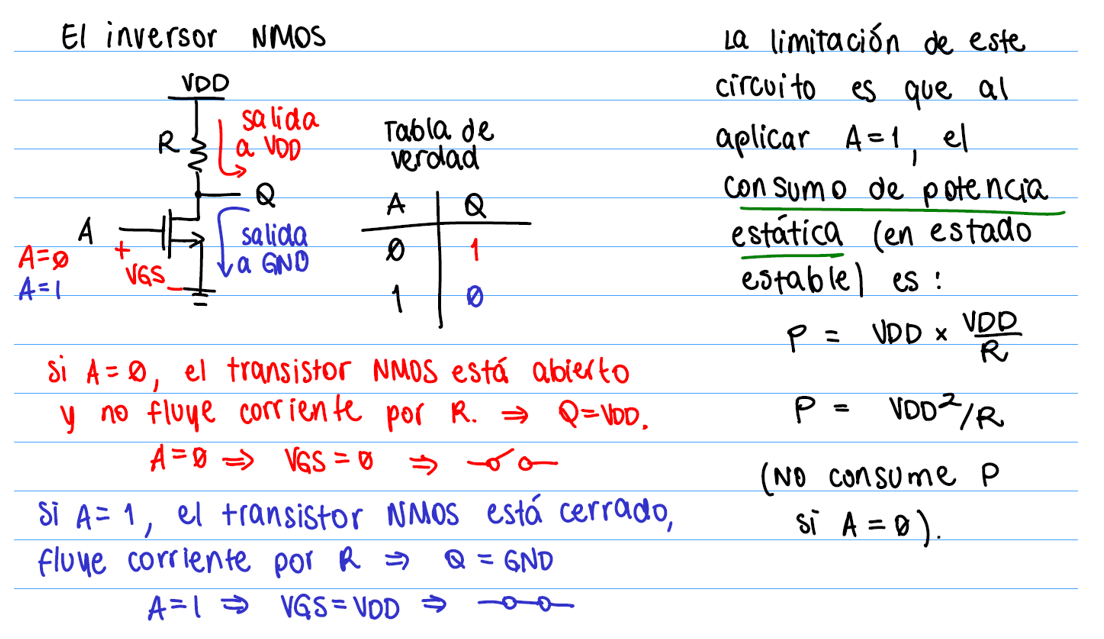
\includegraphics[width=0.9\textwidth]{figuras/inversor_nmos.png}
\end{figure}

\end{frame}


\begin{frame}{El inversor CMOS}

\vspace{-5mm}
\begin{figure}
    \centering
    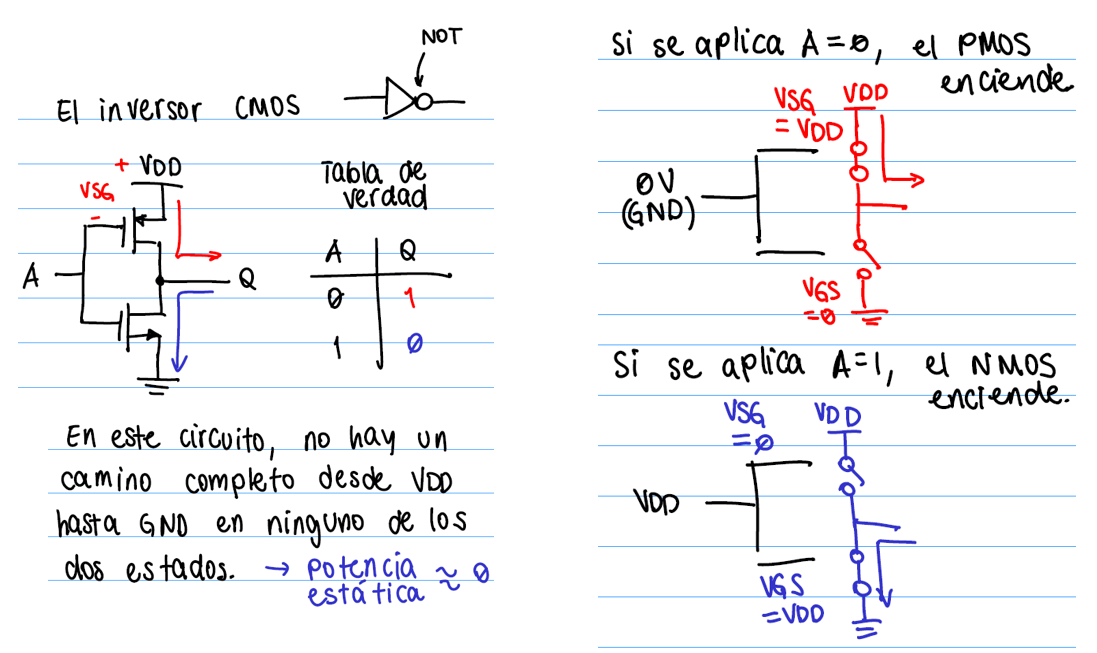
\includegraphics[width=0.9\textwidth]{figuras/inversor_cmos.png}
\end{figure}

\end{frame}



\section{Ejemplo 1}
\begin{frame}{Ejemplo 1: Inversor NMOS ideal}

\begin{columns}

\begin{column}{0.5\textwidth}

Si un inversor NMOS se construye con una resistencia $R_D = 1\ k\Omega$, y la capacitancia total en el nodo de salida es $C_{out} = 1\ nF$, estime el retardo y el tiempo de transición. Asuma que $W/L = 10/0.18$ y que las capacitancias parásitas son cero.

\vspace{5mm}
¿Cuál es la frecuencia máxima de operación de dicho inversor?

\end{column}

\begin{column}{0.5\textwidth}

\begin{figure}[H]
    \centering
    \begin{circuitikz}[arrowmos]
        \draw (0,0) node[nmos](M1){};
        \draw (0,3) to[R,l=$R_D$] (M1.drain);
        \draw (0,3) node[vdd]{$V_{DD}$};
        \draw (M1.source) node[ground]{};
        \draw (0,1) to[short,-o] (3,1);
        \draw (1.5,1) to[C,l=$C_L$] (1.5,-1);
        \draw (1.5,-1) node[ground]{};
        \draw (3,1) node[right]{$Q$};
        \draw (-1.5,0) to[short,o-] (M1.gate);
        \draw (-1.5,0) node[left]{$A$};
    \end{circuitikz}
\end{figure}

\end{column}

\end{columns}

\end{frame}


\begin{frame}{Solución 1: Inversor NMOS ideal}

\vspace{-5mm}
\begin{columns}

\begin{column}{0.5\textwidth}

Se reemplaza el transistor por el modelo equivalente:

\begin{figure}[H]
    \centering
    \begin{circuitikz}[arrowmos]
        \draw (0,0) to[R,l=$R_n$] (0,-1);
        \draw (0,0) to[nos,l_=$sw$] (0,1);
        \draw (0,3) to[R,l=$R_D$] (0,1);
        \draw (0,3) node[vdd]{$V_{DD}$};
        \draw (0,-1) node[ground]{};
        \draw (0,1) to[short,-o] (3,1);
        \draw (1.5,1) to[C,l=$C_L$] (1.5,-1);
        \draw (1.5,-1) node[ground]{};
        \draw (3,1) node[right]{$Q$};
        \draw (-2.5,1) to[short,o-] (-1.5,1);
        \draw (-2.5,1) node[left]{$A$};
        \draw (-1.5,-1) node[ground]{};
        \draw (-1.5,1) to[open,v=$V_{GS}$] (-1.5,-1);
    \end{circuitikz}
\end{figure}

\end{column}

\begin{column}{0.5\textwidth}

La resistencia del transistor:
\[ R_n = 15\ k\Omega \times \dfrac{L}{W} = 270\ \Omega \]

Los tiempos de transición:
\[ t_{LH} = 2.2RC = 2.2\ \mu s \]
\[ t_{HL} = 2.2RC = 594\ ns \]

Los retardos:
\[ t_{PLH} = 0.7RC = 0.7\ \mu s \]
\[ t_{PHL} = 0.7RC = 189\ ns \]

\end{column}

\end{columns}

\end{frame}


\begin{frame}{Solución 1: Simulación}

\begin{figure}
    \centering
    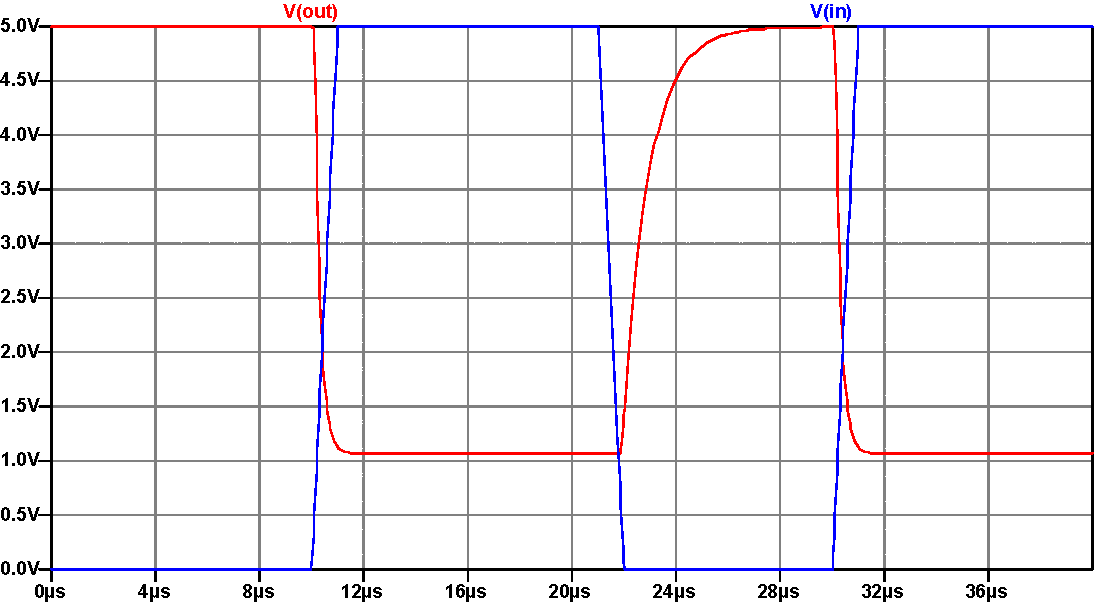
\includegraphics[width=0.8\textwidth]{figuras/inversor_nmos_sim.pdf}
\end{figure}

\end{frame}


\section{Ejemplo 2}
\begin{frame}{Ejemplo 2: Inversor CMOS con capacitancias parásitas}

Dibuje el circuito equivalente de un inversor CMOS incluyendo todas las capacitancias parásitas. Estime el retardo y el tiempo de transición en términos de los parámetros del modelo, suponiendo que el circuito opera sin carga.

\begin{figure}[H]
    \centering
    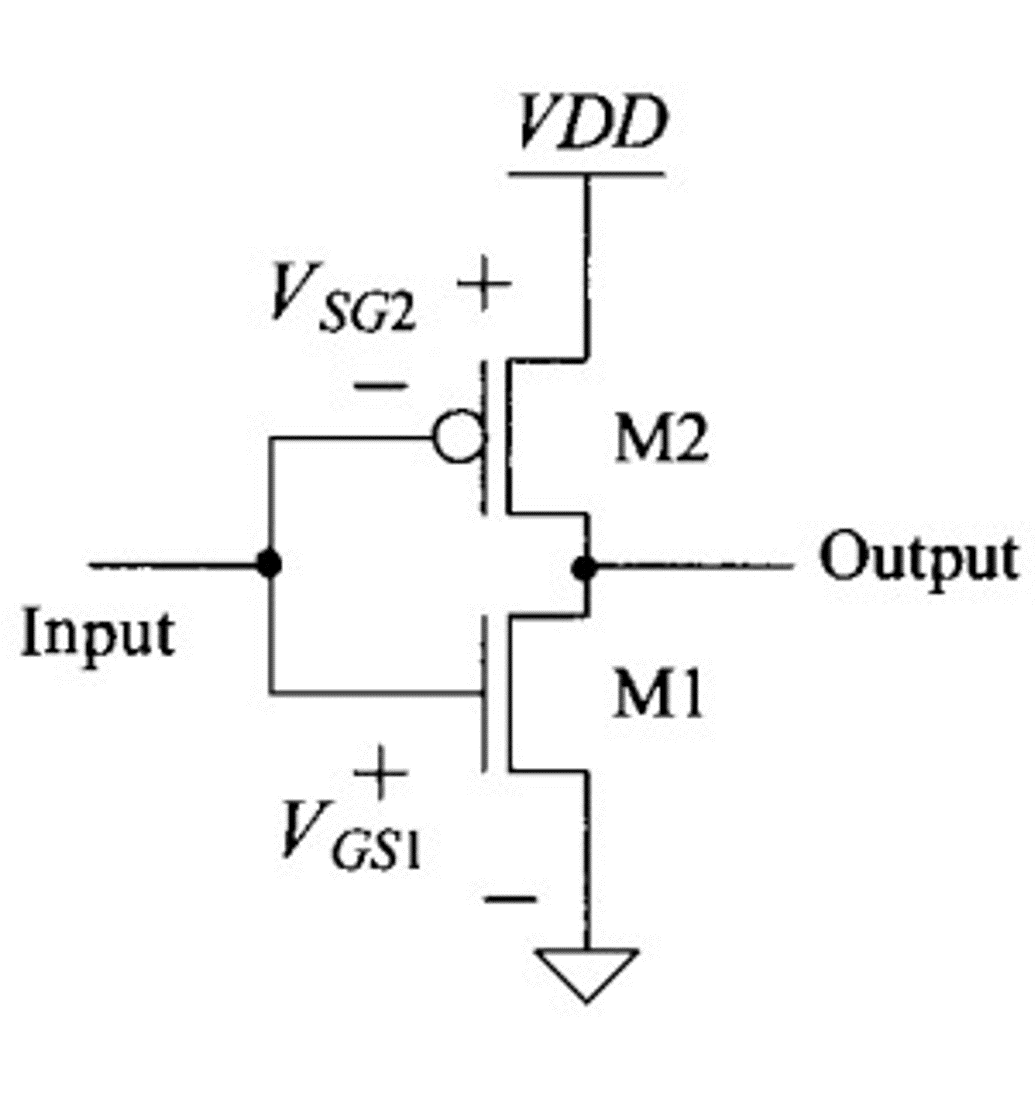
\includegraphics[width=0.3\textwidth]{figuras/inversor_cmos_enunciado.png}
\end{figure}


\end{frame}


\begin{frame}{Solución 2: Inversor CMOS con capacitancias parásitas}

\begin{figure}[H]
    \centering
    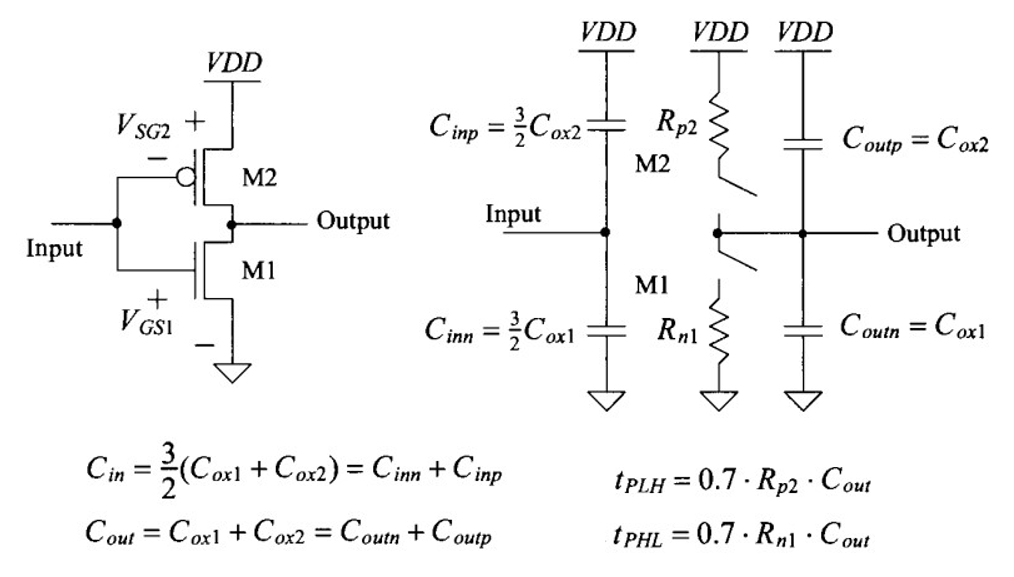
\includegraphics[width=0.8\textwidth]{figuras/inversor_cmos_solucion.png}
\end{figure}

\end{frame}


\section{Referencias}
\begin{frame}{Lecturas recomendadas}

\begin{itemize}
    \item Baker, J. (2019). Chapter 10: Models for Digital Design. In \textit{CMOS: Circuit Design, Layout, and Simulation}, 4th ed., pp. 327-336, Wiley-IEEE Press.
\end{itemize}

\end{frame}


\end{document}
